\documentclass[a4paper, 12pt, oneside]{article}
 
\usepackage[german]{babel}
\usepackage[utf8]{inputenc}
\usepackage[T1]{fontenc}
\usepackage{ae}
\usepackage[table]{xcolor}
\usepackage[bookmarks,bookmarksnumbered]{hyperref}
\usepackage{graphics}
\usepackage{amsmath}           %macht
\usepackage{amsfonts}          %       Mathe
\usepackage{amssymb}           %              mächtiger
\usepackage{graphicx}          %erlaubt Graphiken einzubinden (.eps für dvi und ps sowie .jpg für pdf)
\usepackage[T1]{fontenc}       %Zeichenbelegung der verwendeten Schrift
\usepackage{typearea}	         %ermöglicht änderung des Seitenspiegels
\usepackage{lastpage}          %lässt auf die Seienanzahl zugreifen
\usepackage[margin=10pt,font=small,labelfont=bf]{caption} %macht die Bildbeschriftungen richtig
\usepackage{microtype}
\usepackage{bm}               % bold math, für \bm{}
\usepackage{enumerate}        % verbessert Aufzählungen
\usepackage{array}            % für Tabellen: bindet tabular-Umgebung ein
\usepackage{pdfpages}         % für die Einbindung kompletter pdf-*Seiten*
\usepackage{parskip}          % zw. Absätzen: eine knappe Leerzeile statt hängender Einzüge
\usepackage{dsfont}
\usepackage{tocloft}			% Manipulation des Inhaltsverzeichnisses
\usepackage{siunitx}
\usepackage{parskip}
\usepackage{multirow}
\usepackage{wasysym}
\usepackage{float}
\usepackage{slantsc}
\usepackage{parskip}          % zw. Absätzen: eine knappe Leerzeile statt hängender Einzüge

%%%%%%%%%%%%%%%%%%%%%%%%%%%%%%%%%%%%%%%%%%%%%%%%%%%%%%%%%%%%%%%%%%%%%%%%%%%%%%
%	Abbildungen werden mit Abb. angezeigt.
%
\addto\captionsgerman{%
  \renewcommand{\figurename}{Abb.}%
  \renewcommand{\tablename}{Tab.}%
} 
%
%%%%%%%%%%%%%%%%%%%%%%%%%%%%%%%%%%%%%%%%%%%%%%%%%%%%%%%%%%%%%%%%%%%%%%%%%%%%%%


%%%%%%%%%%%%%%%%%%%%%%%%%%%%%%%%%%%%%%%%%%%%%%%%%%%%%%%%%%%%%%%%%%%%%%%%%%%%%%
%	Kopf- und Fussleiste.
%
\usepackage{fancyhdr}
\fancyhead[LO,LE]{Pflichtenheft -- Iris}
\fancyhead[CO,CE]{}
\fancyhead[RO,RE]{\rightmark}
\fancyfoot[LO,LE]{}

\fancyfoot[CO,CE]{}
\fancyfoot[RO,RE]{\thepage}
%
%%%%%%%%%%%%%%%%%%%%%%%%%%%%%%%%%%%%%%%%%%%%%%%%%%%%%%%%%%%%%%%%%%%%%%%%%%%%%%
 
%%%%%%%%%%%%%%%%%%%%%%%%%%%%%%%%%%%%%%%%%%%%%%%%%%%%%%%%%%%%%%%%%%%%%%%%%%%%%%
%
% Größenanpassungen
%


\usepackage[a4paper]{geometry}
\usepackage{setspace}
\setlength{\unitlength}{1cm}
\setlength{\oddsidemargin}{0.8cm}
\setlength{\evensidemargin}{-0.3cm}
\setlength{\textwidth}{15.5cm}
\setlength{\topmargin}{-1cm}
\setlength{\textheight}{23cm}
\columnsep 0.5cm
\setstretch{1.15} 
%
%%%%%%%%%%%%%%%%%%%%%%%%%%%%%%%%%%%%%%%%%%%%%%%%%%%%%%%%%%%%%%%%%%%%%%%%%%%%%% 
 
\begin{document}
  
\begin{titlepage}
$\,$
\vspace{4cm}\\
\LARGE{Pflichtenheft}
\hrule
\vspace{2cm}

\huge{\textbf{Iris}}\\[1cm]
\Large{\textbf{Version 0.1}}

\vfill
\large
\begin{tabular}{|ll|}
\hline
Autoren: & Daniel Gilgen, Ronny Zingler, Jan Zschoche\\
Datum: & 03.11.2016 \\
Seitenanzahl: & 25\\
\hline
\end{tabular}
\end{titlepage}
 
 
% Platzierung des Inhaltsverzeichnisses
\newpage
\tableofcontents
\pagestyle{fancy}

\newpage
\section{Zielbestimmung}
Dieses Kapitel dient der Bestimmung von Zielen und nicht für deren Verwendung
notwendige Funktionen.
 
\subsection{Musskriterien}
%blubla Musskriterien: Für das Produkt unabdingbare Leistungen, die in jedem Fall
%erfüllt werden müssen \footnote{gezwungen sein, etwas zu tun (Dies ist eine
%beispielhafte Fußnote).}. Das System ist ohne diese Funktionen für seinen
%gedachten Zweck nicht einsetzbar.

Um dem Ziel, der Erkennung einer handegschriebenen Ziffer, gerecht zu werden, müssen 
folgende Kriterien erfüllt sein:

\begin{itemize}
\item Möglichkeit zur Erfassung einer handgeschriebenen Ziffer in einer Weboberfläche
\item Umwandlung der Eingabeziffer in eine maschinenlesbare Form mithilfe neuronaler Netze
\item Ausgabe der Resultate in einer Weboberfläche
\item trainieren der neuronalen Netzten
\item Persistierung von neuronalen Netzen
\end{itemize}
 
\subsection{Kannkriterien}
%Kannkriterien: Die Erfüllung der Kannkriterien ist erwünscht, jedoch nicht
%unbedingt notwendig. Sie sollten nur angestrebt werden, falls noch ausreichend
%Kapazitäten vorhanden sind.

Sind die Musskriterien erfüllt und noch freie Kapazitäten vorhanden, werden folgende Kriterien bearbeitet:

\begin{itemize}
\item Internationalisierung zur Steigerung der Usability
\item Erstellung und Bearbeitung von neuronalen Netzten
\item Bereitstellung der Möglichkeit, verschieden trainierte neuronale Netze auszuwählen
\item Suchfunktion über vorhandene Netze in der Weboberfläche
\end{itemize}

 
\subsection{Abgrenzungskriterien}
Im späteren Entwicklungszyklus der Anwendung sollen die Funktionalitäten erweitert werden. Denkbar wäre die Möglichkeit
der Eingabe einfacher mathematischer Operationen, welche durch das neuronale Netz erkannt und berechnet werden.

\section{Einsatz}
Der geplante Einsatz des Systems ist die Grundlage für Benutzungsoberfläche und
Qualitätsanforderungen.
 
\subsection{Anwendungsbereiche}
%Ein Pflichtenheft wird bspw. in einer IT-Abteilung genutzt.

Das System ist über einen, mit dem Internet verbundenen Rechner aufrufbar.
Dadurch kann die Anwendung von allen Personen mit Internetzugang genutzt werden.


 
\subsection{Zielgruppen}
%Die Zielgruppe besteht also aus Informatikern, die mit der Projektplanung
%beauftragt wurden.

Die größte Zielgruppe ist der Standartnutzer ohne technische Vorkenntnisse, welcher sich für eine Erkennung handschriftlicher Ziffern interessiert.
Da es sich um ein Open-Source Projekt handelt, sollen auch technisch versierte Informatiker angesprochen und zur Teilnahme an der Entwicklung 
der Handschriftserkennung mithilfe neuronaler Netze angeregt werden.

\subsection{Betriebsbedingungen}
%Betriebsbedingungen: Die Betriebsbedingungen spezifiziert die physikalische
%Umgebung des Systems, die tägliche Betriebszeit, und ob das System ständiger
%Beobachtung durch Bediener ausgesetzt ist, oder ein unbeaufsichtigter Betrieb
%beabsichtigt ist.

Die Grundvorrausetzung zur Inbetriebnahme der Anwendung ist ein Server mit Webanbindung. Auf diesem muss mindestens Java 8 installiert sein.
Zur Persistierung der Daten wird mongoDB der Version 3.2.10 verwendet. Der Betrieb der Datenbank muss dauerhaft gewährleistet und die Daten
jederzeit vom Server abrufbar sein. Es wird ein unbeaufsichtiger Betrieb angestrebt. 

 
\section{Umgebung}
 
\subsection{Software}
%Software: Gibt an, welche Software zum Betrieb vorhanden sein muss. Eine
%Aufteilung für Server und Client ist ggf. sinnvoll. Weiterhin sind unbedingt die
%kleinsten benötigten Versionsnummern anzugeben.
\subsubsection {Für Endanwender}

\begin{itemize}
\item aktueller Internet Browser
\end{itemize}

\subsubsection	{Für Entwickler}

\begin{itemize}
\item Java 8
\item Apache Maven 3.3.9
\item Spring Framework 1.4.1
\item Vaadin 7.7.3
\item FasterXML 0.6.2
\item Lombok 1.16.10
\item TestNG 6.9.13.6
\item Mockito 2.0.2 beta
\item dozer 5.5.1
\item Apache Commons-io 2.5
\end{itemize}
 
\subsection{Hardware}

\begin{itemize}
\item Application-Server mit Internetanbindung
\end{itemize} 

\subsection{Orgware}
%Orgware: Angabe der organisatorische Rahmenbedingungen, die vor Projektstart
%erfüllt sein müssen.
\begin{itemize}
\item Web-Repository GitHub zur Versionsverwaltung
\item gitter.im zur internen Kommunikation 
\end{itemize}

\chapter{Funktionalität}
\textcolor{red}{Funktionalität: Spezifikation der einzelnen Produktfunktionen mit genauer und detaillierter Beschreibung.}

Zur Entkopplung einzelner Module und leichteren Wartbarkeit verwendet die Anwendung eine Drei-Schichten Architektur bestehend aus Nutzeroberfläche, Business-Schicht und Daten-Schicht. 
\begin{figure}[h]
\begin{center}
\includegraphics[width=10cm]{Abbildungen/UML/jan/SchichtenModell.png}
\end{center}
\end{figure}
Die Nutzeroberfläche dient der Nutzerinteraktion sowie der Darstellung der Eingabe- sowie verarbeiteten Daten. Sie implementiert dabei das MVP-Muster...

\textcolor{red}{ @Daniel: Hier bitte dein Part für das MVP-Pattern rein!!!}


In der Buisiness-Schicht werden alle fachspezifischen Verarbeitungen vorgenommen. Hierunter fallen beispielsweise die Vorwärtsberechnung sowie das Training eines künstlichen neuronalen Netzes oder die Konvertierung von Daten. Dazu werden für jede Entität spezifizsche Worker-Klassen zur Verfügung gestellt, die diese Aufgaben durchführen können.

\begin{figure}[h]
\begin{center}
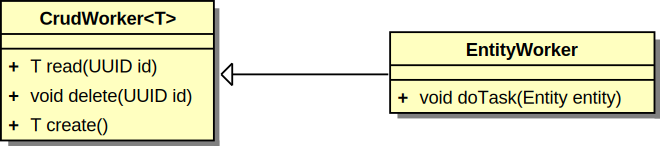
\includegraphics[width=10cm]{Abbildungen/UML/jan/workerClassDiagramm.png}
\end{center}
\end{figure}

Als unterste Schicht der Anwendung dient die Daten-Schicht der Persistierung von Daten. Hierfür stehen ihr diverse, von CRUD-Worker angesprochene Repositories zur Verfügung, die je nach Bedarf Daten (hier im Wesentlichen das Neuronale Netz) in eine Datenbank oder externe Dateien schreiben können.

In den nächsten Unterabschnitten folgt die ausführliche Beschreibung und geplante Umsetzung der von der Anwendung zu erbringenden Funktionalitäten.  


\begin{itemize}
  \item Typische Arbeitsabläufe
  \item Keine Angabe von typischen Verwaltungsfunktionen (CRUD \footnote{Create,
Read, Update, Delete}
\end{itemize}


\section{Training eines Neuronalen Netzes}

\chapter{Produktdaten}

\textbf{/D203/} Für jedes Neuronale Netz werden die folgenden Daten gespeichert: 

\begin{tabular}{cl}
(1) & id \\[0.2cm]
(2) & Name des Neuronalen Netzes\\[0.2cm]
(3) & Beschreibung des Neuronalen Netzes\\[0.2cm]
(4) & Typ Neuronalen Netzwerkes (Prod, Test)\\[0.2cm]
(5) & alle Ids der im Neuronalen Netz enthaltenen Layer.  
\end{tabular}

Für jeden Layer eines Neuronalen Netzes werden die folgenden Daten gespeichert: 

\begin{tabular}{cl}
(1) & id \\[0.2cm]
(2) & Dimension (in x- und y-Richtung) des Layers \\[0.2cm]
(3) & alle Ids der im Layer enthaltenen Knoten.
\end{tabular}

Für jeden Knoten eines Layers werden die folgenden Daten gespeichert: 

\begin{tabular}{cl}
(1) & id \\[0.2cm]
(2) & der Bias \\[0.2cm]
(4) & die Aktivierungsfunktion.
\end{tabular}

Für jedes Kindaxon eines Knotens werden die folgenden Daten gespeichert: 

\begin{tabular}{cl}
(1) & das Gewicht eines Axons \\[0.2cm]
(2) & die Elternknotenid \\[0.2cm]
(3) & die Kindknotenid \\[0.2cm]
\end{tabular}

Zur Persistenz der gesamten oben aufgeführten Daten eines Neuronalen Netzes werden die in Abb. \ref{fig_dbClassdiagram} dargestellten Datenstrukturen verwendet und in einer MongoDB abgelegt. 
\begin{figure}[h]
\begin{center}
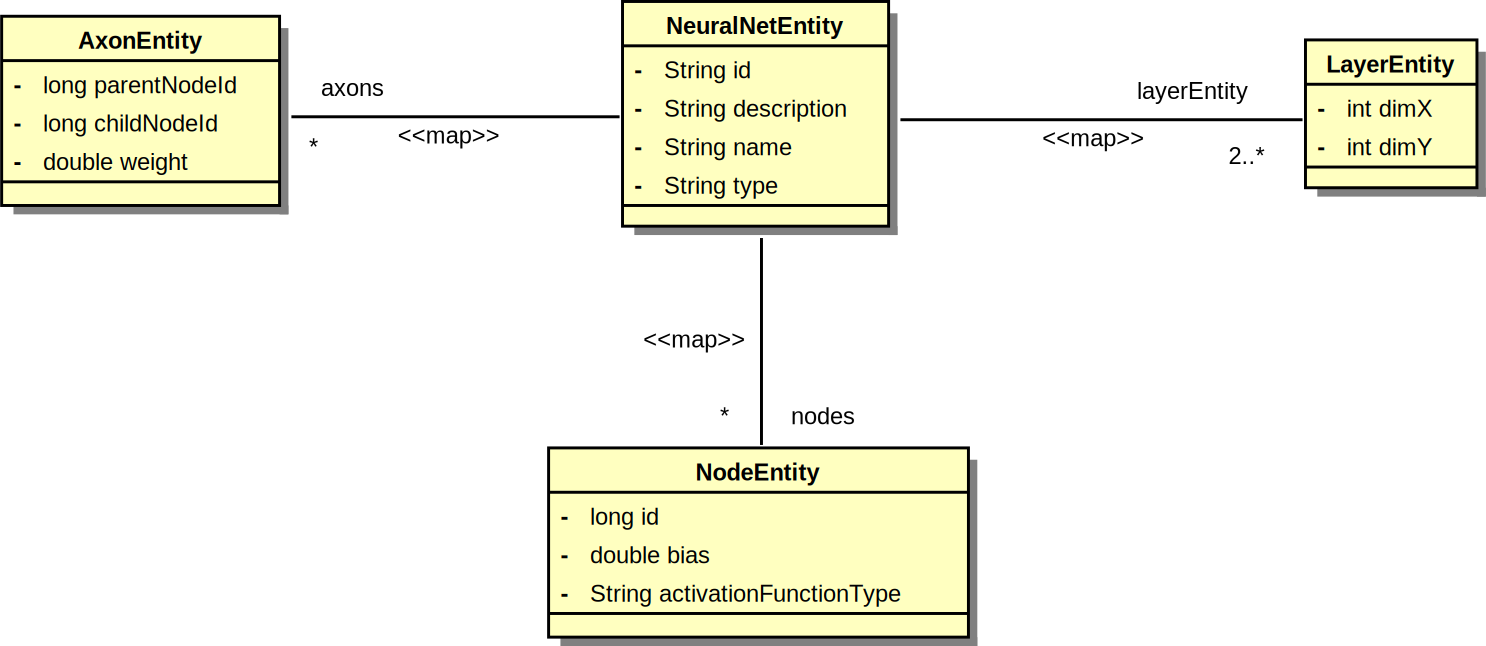
\includegraphics[width=\textwidth]{Abbildungen/UML/jan/datenBankKlassendiagramm.png}
\caption{Klassendiagramm der zur Persistierung eines Neuronalen Netzes benötigten Datenstrukturen.}
\label{fig_dbClassdiagram}
\end{center}
\end{figure}
Es ist zu beachten, dass die Objekt dabei nicht als unabhängige, in Beziehung stehende Entitäten\footnote{Dies entspräche dem Vorgehen für eine Relationale Datenbank. Durch die vielen zirkulären Referenzen ist dieser Zugang nicht geeignet} in der Datenbank sondern als ein einziges Json-Objekt abgelegt werden. 
 
\section{Leistungen}
Anforderungen bezüglich der Zeit und Genauigkeit. \\[-0.2cm]

\textbf{/L101/} Die Webanwendung soll innerhalb weniger Sekunden geladen und einsatzbereit sein. \\[-0.2cm]

\textbf{/L102/} Die in /F102/ beschriebene Berechnung der Ziffer soll in maximal 30ms erfolgen.\\[-0.2cm]

\textbf{/L103/} Die Genauigkeit der Ziffernerkennung soll mindestens 95\% betragen.\\[-0.2cm]

\textbf{/L104/} Die Ausgabe des Ergebnisses soll wahlweise in Echtzeit erfolgen.\\[-0.2cm]

\textbf{/L105/} Die in /F105/ beschriebene Suche soll auch bei vielen Netzen, innerhalb weniger Sekunden, ein Ergebnis liefern.\\[-0.2cm]

\textbf{/L106/} Die in /F106/ beschriebenen Statusinformationen sollen in Echtzeit berechnet und angezeigt werden.\\[-0.2cm]

\textbf{/L201/} Das in /F201/ beschriebene Training soll in maximal textbr{@jan bitte einfügen} abgeschlossen sein.\\[-0.2cm]

\textbf{/L301/} Jede implementierte Funktion soll durch Test auf richtige Funktionsweise überprüfbar sein. Eine Testabdeckung von nahezu 100\% wird angestrebt.\\[-0.2cm]
 
\chapter{Benutzungsoberfläche}
Benutzungsoberfläche: grundlegende Anforderungen, Zugriffsrechte
 
\begin{figure}[ht]
  \centering
  \rule{8cm}{6cm}
  \caption{Dies könnte ein Bild der Benutzungsoberfläche sein}
\end{figure}
 
\section{Qualitätsziele}

\begin{table}[H]
\centering

\label{tabelle_qualitaetsziele}
\begin{tabular}{|lcccc|}
\hline 
\rowcolor[HTML]{E80F9C} %du wolltest es bunt janni ;)
&&&& \\[-0.4cm]
\rowcolor[HTML]{E80F9C}
\textbf{Produktqualität}       & \textbf{sehr gut} & \textbf{gut} & \textbf{normal} & \textbf{nicht relevant} \\[0.1cm]
\hline 
&&&& \\[-0.4cm] 
\textbf{Funktionalität} &&&&   								    		  \\[0.1cm] \hline &&&& \\[-0.4cm]
Angemessenheit        &          & \textbf{x}   &        &                \\[0.1cm]
Richtigkeit           & \textbf{x}        &     &        &                \\[0.1cm]
Interoperabilität     &          & \textbf{x}   &        &                \\[0.1cm]
Ordnungsmäßigkeit     &          &     & \textbf{x}      &                \\[0.1cm]
Sicherheit            &          &     &        & \textbf{x}              \\[0.1cm] \hline &&&& \\[-0.4cm]
\textbf{Zuverlässigkeit} &&&&       							 		  \\[0.1cm] \hline &&&& \\[-0.4cm]
Reife                 &          & \textbf{x}   &        &                \\[0.1cm]
Fehlertoleranz        &          &     & \textbf{x}      &                \\[0.1cm]
Wiederherstellbarkeit &          &     & \textbf{x}      &                \\[0.1cm] \hline &&&& \\[-0.4cm]
\textbf{Bedienbarkeit}&&&&								         		  \\[0.1cm] \hline &&&& \\[-0.4cm]
Verständlichkeit      & \textbf{x}        &     &        &                \\[0.1cm]
Erlernbarkeit         & \textbf{x}        &     &        &                \\[0.1cm]
Bedienbarkeit         & \textbf{x}        &     &        &                \\[0.1cm] \hline &&&& \\[-0.4cm]
\textbf{Effizienz}    &&&&								         		  \\[0.1cm] \hline &&&& \\[-0.4cm]
Zeitverhalten         &          & \textbf{x}   &        &                \\[0.1cm]
Verbrauchsverhalten   &          &     & \textbf{x}      &                \\[0.1cm] \hline &&&& \\[-0.4cm]
\textbf{Änderbarkeit} &&&&						                 		  \\[0.1cm] \hline &&&& \\[-0.4cm]
Analysierbarkeit      & \textbf{x}        &     &        &                \\[0.1cm]
Modifizierbarkeit     &          & \textbf{x}   &        &                \\[0.1cm]
Stabilität            & \textbf{x}        &     &        &                \\[0.1cm]
Prüfbarkeit           & \textbf{x}        &     &        &                \\[0.1cm] \hline &&&& \\[-0.4cm]
\textbf{Übertragbarkeit} &&&&							         		  \\[0.1cm] \hline &&&& \\[-0.4cm]
Anpassbarkeit         & \textbf{x}        &     &        &                \\[0.1cm]
Installierbarkeit     &          &     &        & \textbf{x}              \\[0.1cm]
Konformität           &          &     & \textbf{x}      &                \\[0.1cm]
Austauschbarkeit      &          &     &        & \textbf{x}              \\ \hline
\end{tabular}
\end{table}

\begin{description}
\item[Funktionalität]
Es wird eine leicht bedienbare Weboberfläche gefordert, deren Hauptfunktionen sich intuitiv erschließen.
\item[Zuverlässigkeit]
Die Anwendung soll dem Nutzer über das Internet jederzeit erreichbar sein. Um dies zu erreichen, ist eine hohe Zuverlässigkeit unabdingbar.
\item[Bedienbarkeit]
Um mit der Anwendung umgehen zu können, wird eine Maus und Tastatur benötigt. Die Weboberfläche soll übersichtlich gestaltet sein.
\item[Effizienz]
Die Umwandlung handgeschriebener Ziffern soll in Echtzeit erfolgen. Daraus ergibt sich, dass alle beteiligten Funktionen die Leistungsanforderungen erfüllen müssen
\item[Änderbarkeit]
Durch einen übersichtlichen Quelltext, soll es interessierten Entwicklern möglich sein, die Anwendung weiter zu entwickeln.
\item[Übertragbarkeit]
Da die Anwendung auch ohne Installation ausführbar ist, werden an die Übertragbarkeit keine besonderen Anorderungen gestellt.
\end{description}

 
\newpage 
 
% Abbildungsverzeichnis
\listoffigures
 
\end{document}
